\documentclass{beamer}
\usetheme{Madrid}
\usepackage[T1]{fontenc}
\usepackage{mathpazo}
\usepackage{graphicx}
\usepackage{booktabs}
\usepackage{tikz}
\usetikzlibrary{positioning,arrows.meta,shapes.geometric,fit,backgrounds,calc}
\definecolor{cetnavy}{RGB}{10,26,63}
\definecolor{cetlight}{RGB}{225,231,242}
\setbeamercolor{structure}{fg=cetnavy}
\setbeamercolor{frametitle}{bg=cetnavy,fg=white}
\setbeamercolor{title}{bg=cetnavy,fg=white}
\setbeamertemplate{navigation symbols}{}
% =====================================================================
%  EDIT YOUR DETAILS HERE — this ONE file feeds every abstract & deck.
%  (Change a value, recompile; all 36 documents update.)
% =====================================================================
\newcommand{\seminarName}{Aflah Muhammed P}      % <-- your full name (guessed from your email; please verify)
\newcommand{\seminarRoll}{TVE00CS000}            % <-- your university register/roll number
\newcommand{\seminarClassRoll}{00}               % <-- your class roll no (the short one)
\newcommand{\seminarGuide}{Prof.\ <Guide Name>}  % <-- your guide
\newcommand{\seminarDept}{Department of Computer Science and Engineering}
\newcommand{\seminarCollege}{College of Engineering Trivandrum}
\newcommand{\seminarShortCollege}{CET}           % shown in the slide footer, e.g. "Aflah Muhammed P (CET)"
\newcommand{\seminarShortTitle}{B.Tech Seminar}  % middle of the slide footer
\newcommand{\seminarDate}{July 31, 2026}
% ---------------------------------------------------------------------
% Optional: put a logo image named  cet_logo.png  in this folder and it
% will appear on every title slide automatically. If absent, it is skipped.
% =====================================================================

\title[\seminarShortTitle]{Multi-Agent Collaboration Mechanisms in LLMs: A Survey}
\author[\seminarName\ (\seminarShortCollege)]{\seminarName \\ \seminarRoll \\ Roll No: \seminarClassRoll \\ Guide: \seminarGuide}
\institute[\seminarShortCollege]{\seminarDept \\ \seminarCollege}
\date{\seminarDate}
\titlegraphic{\IfFileExists{cet_logo.png}{\includegraphics[height=1.1cm]{cet_logo.png}}{}}
\begin{document}
\begin{frame}\titlepage\end{frame}
\begin{frame}{Table of Contents}\tableofcontents\end{frame}
\section{Introduction}
\begin{frame}{From Single Models to Collaborating Agents}
\textbf{\textit{Context}}
\begin{itemize}
  \item LLMs now act as autonomous, goal-driven agents.
  \item Complex tasks exceed one model's context and skill.
  \item Groups of agents can coordinate and specialise.
\end{itemize}
\textbf{\textit{This work}}
\begin{itemize}
  \item A survey of \emph{how} LLM agents collaborate.
  \item Reframes the field around collaboration mechanisms.
  \item Tran et al., arXiv:2501.06322, 2025.
\end{itemize}
\end{frame}

\begin{frame}{What is an Agent?}
\begin{itemize}
  \item Agent formalised as $a=\{m,o,e,x,y\}$.
  \item $m$: model; $o$: objective; $e$: environment.
  \item $x$: perceived input; $y$: action, $y=m(o,e,x)$.
  \item Built from profile, memory, planning, action.
\end{itemize}
\end{frame}

\section{Literature Survey}
\begin{frame}{Prior Multi-Agent Frameworks}
\begin{itemize}
  \item \textbf{ChatDev}: simulated software company via chat.
  \item \textbf{MetaGPT}: encodes standard operating procedures.
  \item \textbf{AutoGen}: flexible conversation-driven agents.
  \item \textbf{CAMEL}: role-playing cooperative dialogue.
  \item \textbf{Generative Agents}: memory-based social simulation.
\end{itemize}
\end{frame}

\begin{frame}{Gap in Existing Surveys}
\begin{itemize}
  \item Prior surveys focus on single-agent abilities.
  \item Frameworks described in isolation, ad hoc.
  \item No shared language for collaboration itself.
  \item Hard to compare structures and strategies.
\end{itemize}
\end{frame}

\section{Motivation}
\begin{frame}{Why Study Collaboration Mechanisms}
\begin{itemize}
  \item Collaboration, not scale, unlocks harder tasks.
  \item Specialised roles reduce hallucination and errors.
  \item Debate and review improve reasoning quality.
  \item A unifying view enables reuse and comparison.
  \item Aim: artificial collective intelligence at scale.
\end{itemize}
\end{frame}

\section{Problem Statement}
\begin{frame}{The Problem}
\begin{itemize}
  \item How do LLM agents actually collaborate?
  \item Which design choices govern their interaction?
  \item Existing accounts lack a common taxonomy.
\end{itemize}
\textbf{\textit{Goal}}
\begin{itemize}
  \item Provide an extensible, dimension-based framework.
  \item Organise diverse systems under one lens.
\end{itemize}
\end{frame}

\section{Objectives}
\begin{frame}{Objectives of the Survey}
\begin{itemize}
  \item Define agents and multi-agent systems formally.
  \item Characterise collaboration along five key dimensions.
  \item Map frameworks and real-world applications.
  \item Distil lessons, open challenges, future directions.
\end{itemize}
\end{frame}

\section{Methodology Overview}
\begin{frame}{Five Dimensions of Collaboration}
\begin{center}
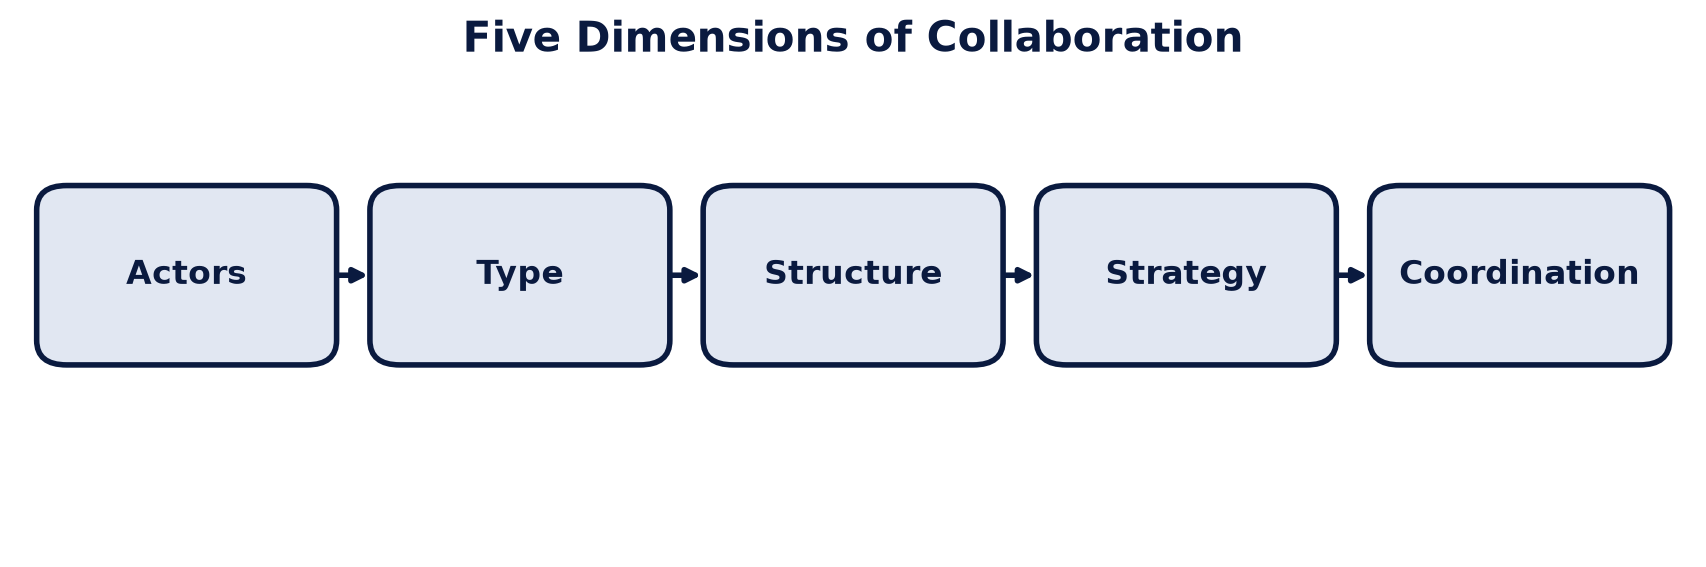
\includegraphics[width=0.9\textwidth,height=0.62\textheight,keepaspectratio]{images/multiagentsurvey_1.png}
\end{center}
\begin{itemize}
  \item Any mechanism = who, how, shape, rule, protocol.
  \item Type: cooperation, competition, or coopetition.
\end{itemize}
\end{frame}

\section{System Architecture}
\begin{frame}{From LLMs to Collective Intelligence}
\begin{center}
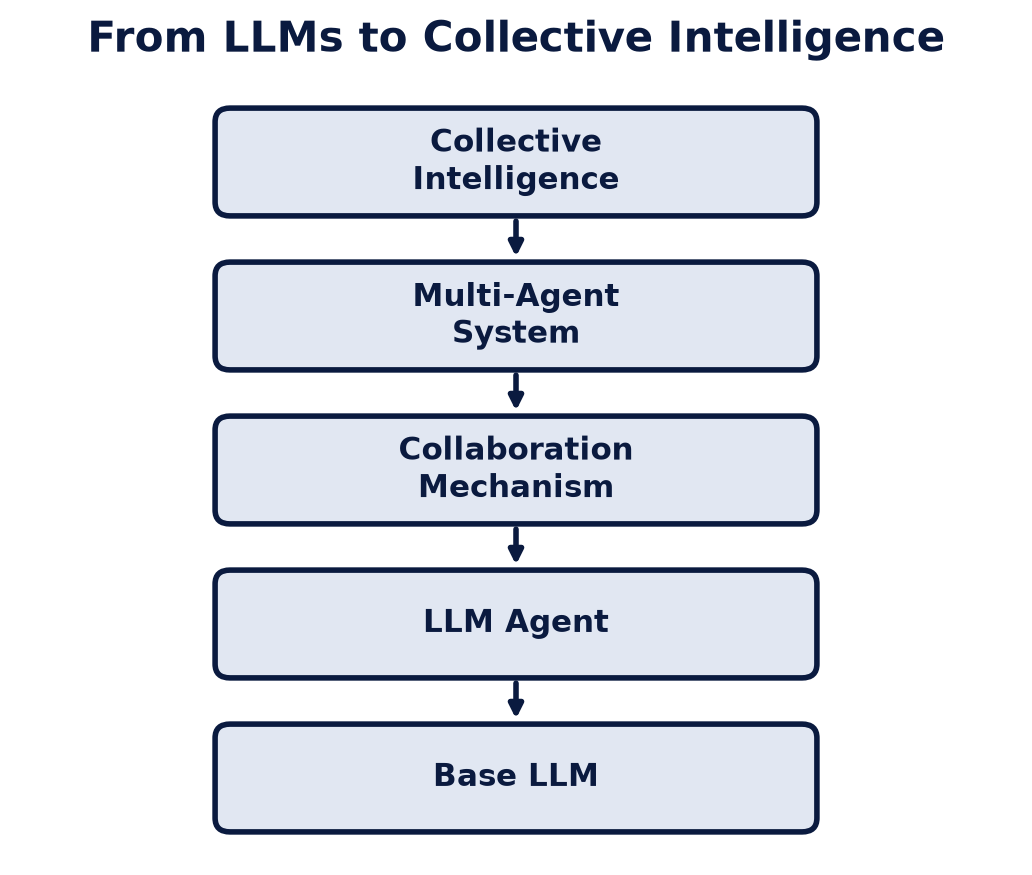
\includegraphics[width=0.9\textwidth,height=0.62\textheight,keepaspectratio]{images/multiagentsurvey_2.png}
\end{center}
\begin{itemize}
  \item Layered view: agents compose into systems.
  \item Mechanism is the bridge to collective behaviour.
\end{itemize}
\end{frame}

\section{Data Collection}
\begin{frame}{Survey Scope and Taxonomy}
\textbf{\textit{Scope}}
\begin{itemize}
  \item LLM-based multi-agent collaboration studies.
  \item Frameworks, protocols, and applied deployments.
\end{itemize}
\textbf{\textit{Organisation}}
\begin{itemize}
  \item Works classified by the five dimensions.
  \item Structures: peer-to-peer, centralized, distributed, hierarchical.
  \item Strategies: rule-based, role-based, model-based.
\end{itemize}
\end{frame}

\section{Model Development}
\begin{frame}{Role-Based Collaboration: A Software Company}
\begin{center}
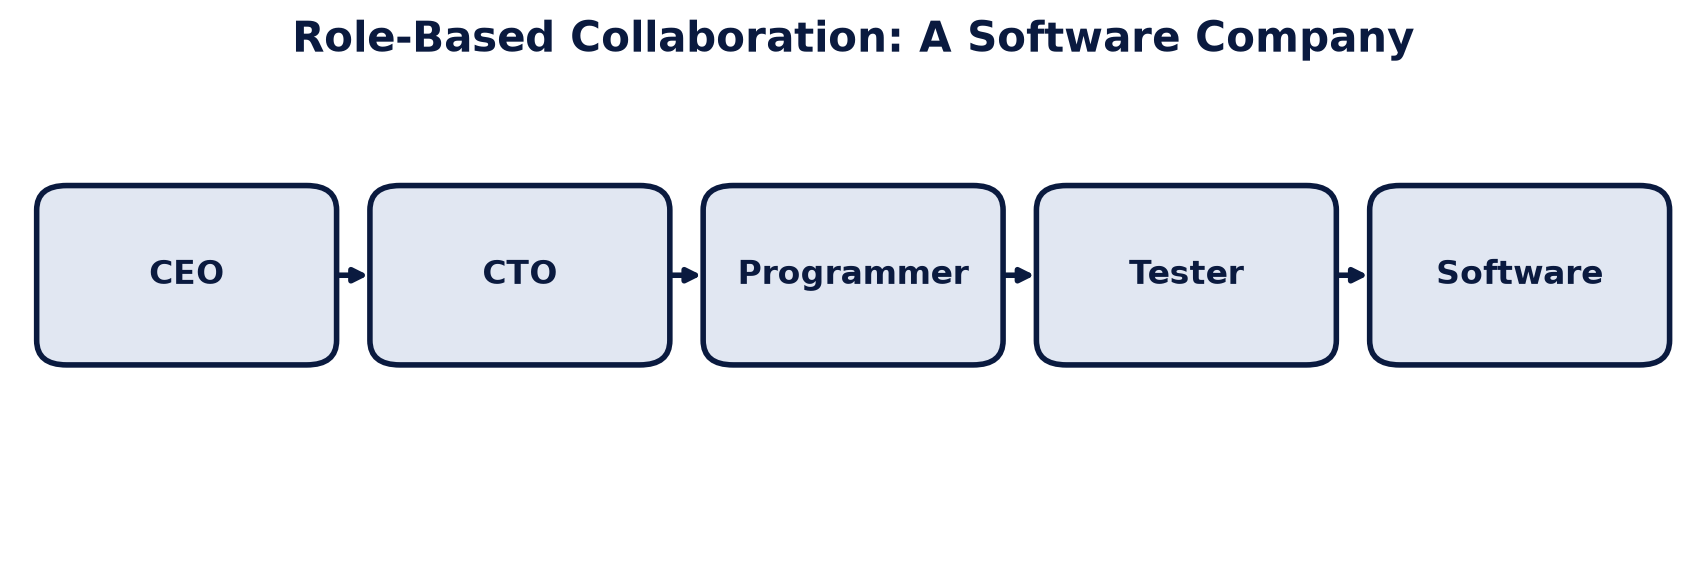
\includegraphics[width=0.9\textwidth,height=0.62\textheight,keepaspectratio]{images/multiagentsurvey_3.png}
\end{center}
\begin{itemize}
  \item Roles assigned; agents talk in natural language.
  \item Cooperation aligns objectives toward one goal.
  \item Competition (debate) and coopetition also studied.
\end{itemize}
\end{frame}

\section{Results}
\begin{frame}{Key Findings of the Survey}
\begin{itemize}
  \item Five dimensions unify diverse MAS designs.
  \item Role-based cooperation dominates practical frameworks.
  \item Structure choice drives scalability and overhead.
  \item Coordination often through natural-language messages.
  \item Emerging use in networks, industry, question answering.
\end{itemize}
\end{frame}

\section{Discussions}
\begin{frame}{Interpretation and Trade-offs}
\begin{itemize}
  \item Specialisation improves quality but adds coordination cost.
  \item Centralized control is simple yet a bottleneck.
  \item Debate boosts reasoning but risks disagreement loops.
  \item Framework is descriptive and extensible, not prescriptive.
\end{itemize}
\end{frame}

\section{Challenges}
\begin{frame}{Open Challenges}
\begin{itemize}
  \item Cascading hallucinations across cooperating agents.
  \item Communication overhead limits scalability.
  \item Lack of standard benchmarks and metrics.
  \item Memory, trust, and safety in long interactions.
  \item Evaluating emergent collective behaviour is hard.
\end{itemize}
\end{frame}

\section{Future Work}
\begin{frame}{Future Research Directions}
\begin{itemize}
  \item Adaptive structures and dynamic role assignment.
  \item Robust coordination protocols and shared memory.
  \item Rigorous benchmarks for collaborative performance.
  \item Human-agent teaming and alignment.
  \item Scaling toward artificial collective intelligence.
\end{itemize}
\end{frame}

\section{Conclusion}
\begin{frame}{Conclusion}
\begin{itemize}
  \item Collaboration is the key to capable agent systems.
  \item Five dimensions give a shared, extensible vocabulary.
  \item Taxonomy maps frameworks and applications coherently.
  \item Clear challenges point toward collective intelligence.
\end{itemize}
\end{frame}

\section{References}
\begin{frame}{References}
\footnotesize
\begin{itemize}
  \item K.-T. Tran, D. Dao, M.-D. Nguyen, Q.-V. Pham, B. O'Sullivan, and H. D. Nguyen, ``Multi-Agent Collaboration Mechanisms: A Survey of LLMs,'' arXiv:2501.06322, 2025.
  \item C. Qian, W. Liu, H. Liu, et al., ``ChatDev: Communicative Agents for Software Development,'' in Proc. ACL, 2024; arXiv:2307.07924.
  \item S. Hong, X. Zheng, J. Chen, et al., ``MetaGPT: Meta Programming for a Multi-Agent Collaborative Framework,'' in Proc. ICLR, 2024; arXiv:2308.00352.
\end{itemize}
\end{frame}
\begin{frame}\vfill\centering{\Huge Thank You}\vfill\end{frame}
\end{document}
